\documentclass{article}

\usepackage{amsmath}
\usepackage{amssymb}
\usepackage[utf8]{inputenc}
\usepackage{graphicx}
\usepackage[english]{babel}
\usepackage[T1]{fontenc}
\usepackage{lmodern,mathrsfs}
\usepackage{xparse}
\usepackage[inline,shortlabels]{enumitem}
\setlist{topsep=2pt,itemsep=2pt,parsep=0pt,partopsep=0pt}
\usepackage[dvipsnames]{xcolor}
\usepackage[utf8]{inputenc}
\usepackage[most]{tcolorbox}
\tcbuselibrary{minted} % tcolorbox minted library, required to use the "minted" tcb listing engine (this library is not loaded by the option [most])
\usepackage{minted} % Allows input of raw code, such as Python code
\usepackage[colorlinks]{hyperref} % ALWAYS load this package LAST
\tcbset{
    pythoncodebox/.style={
        enhanced jigsaw,breakable,
        colback=gray!10,colframe=gray!20!black,
        boxrule=1pt,top=2pt,bottom=2pt,left=2pt,right=2pt,
        sharp corners,before skip=10pt,after skip=10pt,
        attach boxed title to top left,
        boxed title style={empty,
            top=0pt,bottom=0pt,left=2pt,right=2pt,
            interior code={\fill[fill=tcbcolframe] (frame.south west)
                --([yshift=-4pt]frame.north west)
                to[out=90,in=180] ([xshift=4pt]frame.north west)
                --([xshift=-8pt]frame.north east)
                to[out=0,in=180] ([xshift=16pt]frame.south east)
                --cycle;
            }
        },
        title={#1}, % Argument of pythoncodebox specifies the title
        fonttitle=\sffamily\bfseries
    },
    pythoncodebox/.default={}, % Default is No title
    %%% Starred version has no frame %%%
    pythoncodebox*/.style={
        enhanced jigsaw,breakable,
        colback=gray!10,coltitle=gray!20!black,colbacktitle=tcbcolback,
        frame hidden,
        top=2pt,bottom=2pt,left=2pt,right=2pt,
        sharp corners,before skip=10pt,after skip=10pt,
        attach boxed title to top text left={yshift=-1mm},
        boxed title style={empty,
            top=0pt,bottom=0pt,left=2pt,right=2pt,
            interior code={\fill[fill=tcbcolback] (interior.south west)
                --([yshift=-4pt]interior.north west)
                to[out=90,in=180] ([xshift=4pt]interior.north west)
                --([xshift=-8pt]interior.north east)
                to[out=0,in=180] ([xshift=16pt]interior.south east)
                --cycle;
            }
        },
        title={#1}, % Argument of pythoncodebox specifies the title
        fonttitle=\sffamily\bfseries
    },
    pythoncodebox*/.default={}, % Default is No title
}
\newtcolorbox{pythonbox}[1][]{pythoncodebox=#1}
\newminted{python}{autogobble,breaklines,mathescape}
\NewTCBListing{python}{ !O{} !D(){} !G{} }{
    listing engine=minted,
    listing only,
    pythoncodebox={#1}, % First argument specifies the title (if any)
    minted language=python,
    minted options/.expanded={
        autogobble,breaklines,mathescape,
        #2 % Second argument, delimited by (), denotes options for the minted environment
    },
    #3 % Third argument, delimited by {}, denotes options for the tcolorbox
}
\usepackage{parskip}
\usepackage{amsthm}
\usepackage{indentfirst}
\setlength{\parindent}{0.3cm}
\setlength{\parskip}{0.2cm}
\linespread{1.2}
\usepackage{amsthm}
\theoremstyle{definition}
\newtheorem{example}{Example}[section]

\usepackage{geometry}
 \geometry{
 a4paper,
 total={170mm,257mm},
 left=30mm,
 right=30mm,
 top=30mm,
 bottom=30mm
 }

\begin{document}


\title{Boot camp for RESCEU KAGRA project}
\author{Seonjun Kwon}
\date{RESCEU, Department of Physics, The University of Tokyo}
\maketitle
\tableofcontents

\newpage
\section{Basic Settings}

We assume that you use LINUX OS.

There are many packages for Python language which CANNOT be used in Windows environment.

In this section, you can learn how to install packages, revise programs, etc..

\subsection{LINUX}

\subsubsection{Start LINUX}

Open terminal. You can see that for example for me,

\begin{verbatim}
    seonjunkwon@resceuX13:~$
\end{verbatim}

Of course your name and your machine's name are different from mine; The important thing is that you can enter command after the symbol \$.

The window of this terminal you are seeing now is your home directory.

\subsubsection{Directory}

Doing all thing in home directory is NO-efficient. So, we need to move to directory we use.

Open terminal, enter command below.

\begin{verbatim}
    $ cd Documents/
\end{verbatim}

Tip: Enter Docu and push Tab-key, you can write 'Documents' more easily.

You moved to Documents directory.

Next, check the recent directory.

After \# is annotation.

\begin{verbatim}
    $ ls # Check what is in this directory
    $ ls / # See root directory
    $ ls .. # See the directory above a step
    $ ls ~ # See home directory
    $ ls -a # See all files including hidden files
    etc.
\end{verbatim}

For more information and more options, please enter

\begin{verbatim}
    $ ls -help
\end{verbatim}

We can make/remove the directory(file).

\begin{verbatim}
    $ mkdir NewDirectory # Make an empty directory
    $ rmdir NewDirectory # Remove an EMPTY directory
    $ rm -rf NewDirectory # Remove a directory and all the files in which
\end{verbatim}

With rmdir, we can remove empty directory only. If you want to remove a directory in which files exist, you can use 'rm -rf'.

We can make/remove a test file.

\begin{verbatim}
    $ vi test.txt # Make an empty text file
\end{verbatim}

You will enter to VI. Type ':wq' to exit(make an empty file).

\begin{verbatim}
    $ mkdir TestDirectory # Make a directory
    $ mv test.txt TestDirectory # Move test file to TestDirectory
    $ vi test2.txt
     # Make a new empty text file: In VI, please type ':wq' and enter(return).
    $ mv test2.txt renamed.txt # Rename test2.text to renamed.txt
    $ mv TestDirectory/test.txt ./
     # Move test.txt in TestDirectory to current directory
    $ cp test.txt TestDirectory/ # Copy text.txt to TestDirectory
\end{verbatim}

You can make, move and copy a file.

\subsection{VI}

\subsubsection{Start VI}

VI has command mode, visual mode and insert mode.

Turn on a terminal and make a file.

\begin{verbatim}
    $ vi text.txt
\end{verbatim}

(If there exists text.txt, we can revise that file.)

The terminal will be changed to VI editor, especially command mode.

In command mode, you can enter to visual mode by entering below.

\begin{verbatim}
    v : Enter to visual mode (Select per letters)
    V : Enter to visual line mode (Select per sentences)
\end{verbatim}

You can go back to command mode by enteing 'esc' key.

In command mode, you can enter to insert mode by entering (1 of) those commands.

\begin{verbatim}
    a : Enter from the next letter of cursor
    A : Enter from the end of this column
    i : Enter from the previous letter of cursor
    I : Enter from the start of this column
    o : Enter with empty column under this column
    O : Enter with empty column above this column
    s : Enter deleting a letter on cursor
\end{verbatim}

In insert mode, you can go back to command mode by entering 'esc' key.

You can save the file and exit VI command mode, and go back to terminal by entering below.

\begin{verbatim}
    :wq
\end{verbatim}

\subsubsection{Command Mode}

For more information, enter below IN TERMINAL.

\begin{verbatim}
    $ vi -h
\end{verbatim}

In command mode in VI, we can use move keys, especially

\begin{verbatim}
    h : left key
    j : down key
    k : up key
    l : right key
    w : Move to the next word
    b : Move to the previous word
    gg : Move to the first column
    G : Move to the last column
    ( : Move to the previous sentence
    ) : Move to the next sentence
    { : Move to the pervious paragraph
    } : Move to the next paragraph
    etc.
\end{verbatim}

You can delete column(s) by

\begin{verbatim}
    dd : Delete this column
    d3 : Delete 3+1=4 columns
    etc.
\end{verbatim}

You can copy and paste column(s) by

\begin{verbatim}
    yy : Copy this column
    y5 : Copy 5+1=6 columns
    p : Paste next to cursor
    P : Paste in front of cursor
    etc.
\end{verbatim}

And you can do below.

\begin{verbatim}
    /[word] : Find [word]
    n : Next find result
    u : Undo
    [ctrl] r : Redo
    etc.
\end{verbatim}

You can check and use another convenient methods to revise files by

\begin{verbatim}
    $ vi -h
\end{verbatim}

\subsubsection{Visual Mode}

You can enter visual mode from command mode, by entering

\begin{verbatim}
    v
\end{verbatim}

You can select from the cursor position before entering visual mode.

\begin{verbatim}
    [Arrow keys] : Select an area
    ~ : Convert the letter type and go back to command mode;
    big to small or small to big
    d : Delete the area and go back to command mode
    c : Delete the area and ENTER TO INSERT MODE
    y : Copy the area and go back to command mode
    [esc] : Do nothing and go back to command mode
\end{verbatim}

\subsubsection{Insert Mode}

You can revise the file in insert mode, and this is almost same as that of Windows memo or wordpad.

\subsection{SSH}

\subsubsection{Create an Account}\label{SSH}

Using SSH, you can enter to the supercomputer, RESCEUBBC or IGWN computer, etc. for example.

At first, talk to your supervisor and create your account. If you received email about SSH, please follow that guideline.

If you want to have your own SSH key(public and private), open the terminal and enter below.

\begin{verbatim}
    $ ssh-keygen
\end{verbatim}

SSH keys are stored in the '$\sim$/.ssh' folder.

You will have 'id\_rsa' file or 'id\_ed25519' file and that's '.pub' file. The file '.pub' is a public file, and the file without an extension is a private file. You should not disclose your private file to anyone other than yourself. The file to be uploaded to the authentication website is also a public file, so you do not need to upload a private file. The private file on your computer is used to log in using SSH, with the public file uploaded to the authentication website.

\subsubsection{Login}

In terminal, enter below.

\begin{verbatim}
    $ ssh [account name]@[address]
    $ ssh seonjun.kwon@resceubbc.resceu.s.u-tokyo.ac.jp # for example
\end{verbatim}

You can login with your own password, or public-private keys.

For various options, you can enter below, but I think it is necessary without any options.

\begin{verbatim}
    ssh
    scp help
\end{verbatim}

\subsubsection{Upload and Download}

You can upload and download the file or directory with 'scp'.

In local terminal,

\begin{verbatim}
    $ scp [file] [account name]@[address]:[target directory] # Upload a file
    $ scp -r [directory] [account name]@[address]:[target directory]
     # Upload a directory
    $ scp [account name]@[address]:[directory]/[file] [Downloading directory]
     # Download a file
\end{verbatim}

\subsection{GIT}

You can upload your files to GIT in order for your colleagues to see and check the file, and also you can download the file from your GIT. It is very useful for your remote works.

\subsubsection{Initial Settings}

Talk to your supervisor, and make your git address for your thesis. It should have the 'readme.md' file.

After that, you should do a little work in local.

In your local computer, you should make a local directory to share your file.

\begin{verbatim}
    $ mkdir gitshare
\end{verbatim}

You can set the directory name for your own, not only 'gitshare'.

Make an initial environment.

\begin{verbatim}
    $ cd gitshare
    ~gitshare/$ git init
    ~gitshare/$ git remote add origin [Your git address]
    ~gitshare/$ git branch -M main
    ~gitshare/$ git push -u origin main
\end{verbatim}

Once you added the remote address, you don't have to add the remote git address.

You have to check your git's branch,

\begin{verbatim}
    ~gitshare/$ git branch
\end{verbatim}

You can see your all branch, and the branch with '*' is the branch selected.

You can make a branch and change the selected branch.

\begin{verbatim}
    ~gitshare/$ git branch [branch name] # Make a branch
    ~gitshare/$ git checkout -b [branch name]
     # Checkout from the branch and make a new branch
    ~gitshare/$ git branch -d [branch name] # Delete a branch
\end{verbatim}

For more information, you can see \href{https://git-scm.com/book/en/v2}{Git book}.

\subsubsection{Upload}

First, you should 'add' your file and second 'commit', and push(means upload) the committed file.

\begin{verbatim}
    ~gitshare/$ git add [file name] # Upload a file
    ~gitshare/$ git add .
     # Upload all files, CAUTION FOR THIS COMMAND!!
       IF THERE DOESN'T EXISTS THE FILE IN LOCAL, THAT EXISTS IN GIT,
       THE FILE WILL BE DELETED.
    ~gitshare/$ git commit -m [message] # Commit
    ~gitshare/$ git push # Push
    ~gitshare/$ git push -f # Push forcely
\end{verbatim}

For more information, you can see \href{https://git-scm.com/book/en/v2}{Git book}.

\subsubsection{Download}

You can download(merge) files from git to local.

\begin{verbatim}
    ~gitshare/$ git pull # Pull(Download), it can occur an error.
    ~gitshare/$ git pull -f
     # Pull forcely,
       IF YOU ARE CONFIDENT THAT
       YOU CAN CHANGE ALL YOUR LOCAL FILES TO THAT IN GIT.
\end{verbatim}

You can undo your previous commitments, add tag, fetch forcely, etc.. For those information, you can see \href{https://git-scm.com/book/en/v2}{Git book}.

\subsubsection{Set the Access Token}

You can set the access token, and SHOULD set it if you are using Github.

LIGO git: Go to the "User Settings - Access tokens". And then click "Add new token" and set the token's name, expire date, and the scopes(permissions).

Github: Go to your profile and enter "Settings - Developer settings". Enter "tokens(classic)" and click "Generate new token". Set the token's name, expire date, and the permissions.

You have to save the token in your own storage: this should not be leaked. If not saved, you cannot see the token so you have to regenerate a token.

And then set the remote path.

\begin{verbatim}
    ~gitshare/$ git remote hub https://<Username>:<Token>@github.com/<Address>.git
\end{verbatim}

If you are using LIGO git, it is almost same.
\begin{verbatim}
    ~gitshare/$ git remote origin https://<Username>:<Token>@git.ligo.org/<Address>.git
\end{verbatim}

Then, you can copy and link your project in LIGO git to github, which does not expire even if you graduate. (We assume that the local path is 'gitshare'.)

\begin{verbatim}
    $ git pull origin main
    $ git push hub main
\end{verbatim}

If you worked locally,

\begin{verbatim}
    $ git add .
    $ git commit -m "<Your commit message>"
    $ git push origin main
    $ git push hub main
\end{verbatim}

Caution: Uploading a file over 100MB in Github is very annoying. Make sure to check if you have files over 100MB in size locally.

\subsection{Conda and Python}

When you are doing research, you should make a program for your research, using Python3.

\subsubsection{Download Conda}

First, download installation file.

\begin{verbatim}
    $ wget https://repo.anaconda.com/archive/Anaconda3-2024.06-1-Linux-x86_64.sh
\end{verbatim}

I recommend to download the newest version.

Run the installation file.

\begin{verbatim}
    bash Anaconda3-2024.06-1-Linux-x86_64.sh
\end{verbatim}

We have to set the path.

\begin{verbatim}
    $ source ~/.bashrc
    $ vi ~/.bashrc
\end{verbatim}

In VI, you add

\begin{verbatim}
    export PATH="/home/username/anaconda3/bin:$PATH"
\end{verbatim}

where 'username' is your user name.

\subsubsection{Use Python 3.10 with Conda}

I recommend the Python version 3.10, and you can also use another version of Python.

Let's create a virtual environment.

\begin{verbatim}
    $ conda create -n python3.10 python=3.10
\end{verbatim}

We can see that
d
\begin{verbatim}
    Proceed ([y]/n)?
\end{verbatim}

Type y.

You can see the environments using below.

\begin{verbatim}
    $ conda info -e
\end{verbatim}

To run python file, you have to activate the python environment.

\begin{verbatim}
    $ conda activate python3.10
\end{verbatim}

\subsubsection{Set Path}

You have to set path to run your package. It can be set automatically, but if not, you cannot run the package you installed.

PLEASE DO THIS SECTION ONLY IF AN ERROR OCCURED IMPORTING DOWNLOADED PACKAGE. If it works without any path settings, you can move to next section.

PLEASE ASK YOUR SUPERVISOR OR LINUX EXPERT ABOUT THAT PROBLEM IF YOU DON'T HAVE A CONFIDENCE.

If you use local, you have to check where is your Python. And edit '.bashrc' file.

\begin{verbatim}
    $ which python3
    $ vi .bashrc
\end{verbatim}

In VI, you can add that phrase in the bottom of that file,

\begin{verbatim}
    export PATH=[Your Python path]:$PATH
\end{verbatim}

If you made a mistake, a temporarily solution is to enter this phrase in the bottom of that file.

\begin{verbatim}
    export PATH=$(getconf PATH)
\end{verbatim}

AND PLEASE ASK YOUR SUPERVISOR OR LINUX EXPERT.

\subsubsection{Install Packages}

We have to install the necessary packages.

\begin{verbatim}
    $ conda activate python3.10
    $ pip install numpy matplotlib bilby gwpy pycbc
\end{verbatim}

And the 'argparse' package will help you to do testing and running file, or multi-processing.

\begin{verbatim}
    $ pip install argparse
\end{verbatim}

If you have to install more packages, please install WITH CONDA, not pip.

\begin{verbatim}
    $ conda install -n python3.10 [package-name]
\end{verbatim}

If this doesn't work,

\begin{verbatim}
    $ conda install -n python3.10 -c conda-forge [package-name]
\end{verbatim}

When we have to install a specific version of the package, we can use version number. for example, 

\begin{verbatim}
    $ pip install numpy==1.14.5
    $ conda install tensorflow=2.5
\end{verbatim}

You can see we have 2 =s in pip, and 1 = in conda.

For more information about pip and conda,

\begin{verbatim}
    $ pip help
    $ conda
\end{verbatim}

\subsubsection{Python Tutorial}

You have to study Python before make your own program.

We consider you to have a basic knowledge of the Python language. If not, please see and study  \href{https://docs.python.org/3/tutorial/index.html}{Python Tutorial}.

\subsubsection{Run .py File}

You can run your own Python file you made.

\begin{verbatim}
    $ python3 test.py
\end{verbatim}

If you set your Python as 'python3.10' not 'python3'(especially for example Conda environment), you can run with

\begin{verbatim}
    $ python3.10 test.py
\end{verbatim}

\subsubsection{Make a Program}

You can run a file, which isn't '.py' file. For example, take that the file name is 'test', not 'test.py'.

In the first of file, you have to add

\begin{verbatim}
    #!/usr/bin/env python3
\end{verbatim}

And run the file

\begin{verbatim}
    $ ./test
\end{verbatim}

The running language will be Python 3.

\subsubsection{Argparse Packge}

You can run a file with various options using argparse package.

Make a file(with Python language). For convenient, the file name will be 'test'.

\begin{python}[python3]
    #!usr/bin/env python3
    
    # Set initial environment
    import argparse
    parser = argparse.ArgumentParser(
        prog = 'ProgramName',
        description = 'What the program does',
        epilog = 'Text at the bottom of help')
    parser.add_argument('-c',
                        '--count',
                        type=int,
                        default=1,
                        help='The number of simulation times')
    args = parser.parse_args()

    # Define a function
    def run(n):
        print(n)
    for n in range(args.count):
        run(n)
\end{python}

And print from 1 to 10.

\begin{verbatim}
    $ ./test -c 10
\end{verbatim}

Of course, you can run with entering this command,

\begin{verbatim}
    $ python3 test -c 10
\end{verbatim}

You can use this package for other purposes, and for more information, you can see \href{https://docs.python.org/3/howto/argparse.html}{Argparse Tutorial}.

\subsubsection{Nohup and Tail}

Using 'nohup', you can activate a program in background, when you have to logout from ssh server.

\begin{verbatim}
    $ nohup python3.10 test.py &
\end{verbatim}

If you didn't enter '\&', the program is activated in foreground, so if you have to logout during the program running, you have to type '\&' at the last of the command.

If the program is running in foreground, you cannot interact with the shell(terminal) until the end of the running.

'tail' prints the last 10 lines of each file to standard output.

To see the last 10 lines of the nohup file, you can enter below.

\begin{verbatim}
    $ tail nohup.out
\end{verbatim}

If you want to see the status in real time, you can enter the following.

\begin{verbatim}
    $ tail -f nohup.out
\end{verbatim}

Of course, this state can escape by entering Ctrl-c.

If you did multi-processing so nohup says nothing, you can use 'nohup' and '-u'. For example,

\begin{verbatim}
    $ nohup python3.10 -u test.py &
\end{verbatim}

For more information about 'tail', you can type that

\begin{verbatim}
    $ tail --help
\end{verbatim}

\subsection{Data Access}

\subsubsection{GWOSC}

\subsubsection{O4 data}
\section{Mathematics, Physics, and Statistical Methods}

\subsection{Mathematics}

\subsubsection{Gaussian Distribution}

The probability density function of Gaussian distribution is as follows, where $\mu$ is the mean and $\sigma$ is the standard deviation.

\begin{equation}
    \mathrm{N}(\mu, \sigma^2): \quad \frac{1}{\sigma\sqrt{2\pi}} \exp{\left(-\frac{(x - \mu)^2}{2 \sigma^2} \right)}
\end{equation}

So, we can see that the log of that is a quadratic function.

\begin{equation}
    \ln{P(x)} = -\frac{(x - \mu)^2}{2 \sigma^2} - \ln{\sigma} - \frac{1}{2} \ln{2\pi}
\end{equation}

For more information, please move into \href{https://en.wikipedia.org/wiki/Normal_distribution}{Wikipedia: Normal Distribution}.

\subsubsection{Chi Distribution}

The chi distribution is a probability distribution with positive real numbers as its domain. We have to distinguish between this and the chi-square distribution.

When $k$ variables $x_k$ have a standard normal distribution, we define that the following value $y$ has a $k$-degree chi distribution.

\begin{equation}
    y = \sqrt{\sum_{i=1}^k x_i^{\ 2}}
\end{equation}

Two famous examples are the Rayleigh distribution as a 2-degree chi distribution and the Maxwell-Boltzmann distribution as a 3-degree chi distribution.

The probability density distribution is as follows.

\begin{figure}[h]
\centering
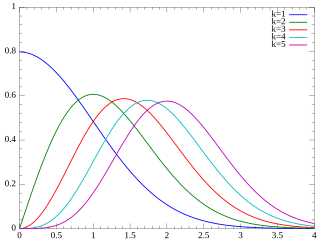
\includegraphics[width=0.5\textwidth]{figs/chi.png}
\caption{The probability density function of chi-distribution.}
\end{figure}

\begin{equation}
    f(x;k) = \frac{x^{k-1} e^{-x^2/2}}{2^{(k/2) - 1} \Gamma(k/2)} \quad (x>0)
\end{equation}

For more information such as cumulative distribution function, visit \href{https://en.wikipedia.org/wiki/Chi_distribution}{Wikipedia: Chi Distribution}.

\subsubsection{Spherical Coordinate System}

To exhibit an isotropic distribution, an understanding of the spherical coordinate system is required.

\begin{figure}[h]
\centering
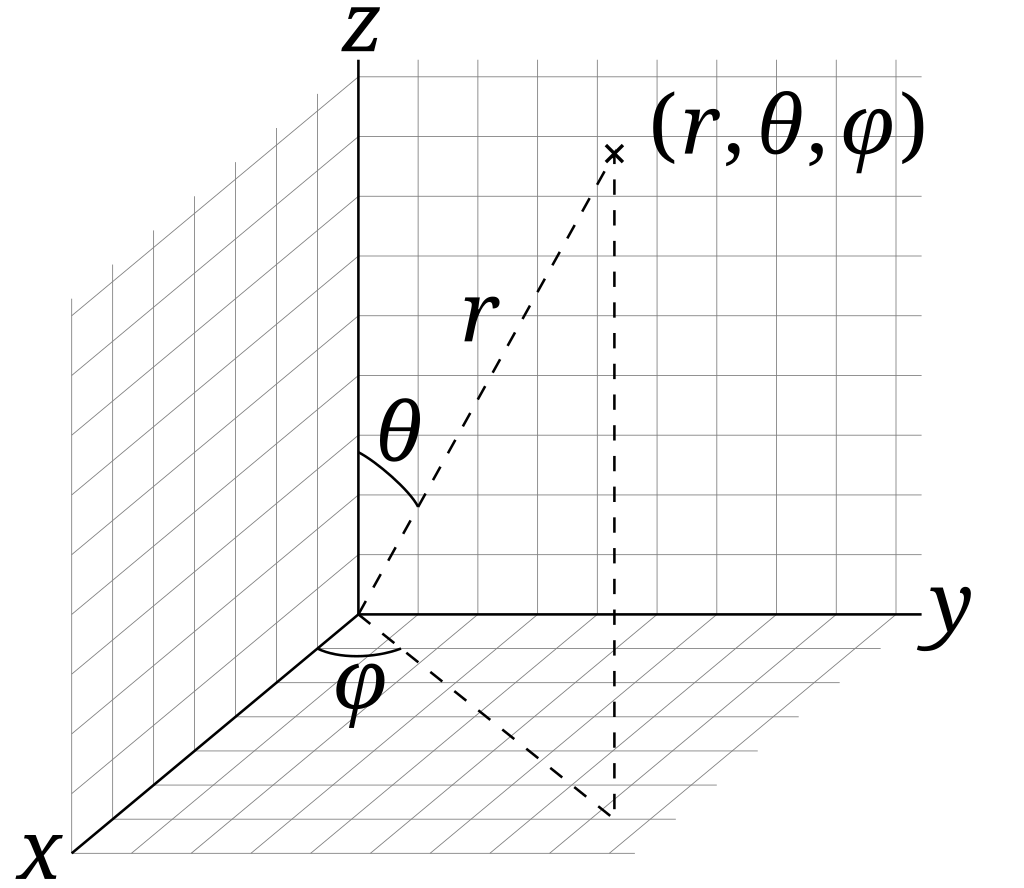
\includegraphics[width=0.5\textwidth]{figs/sphe.png}
\caption{Spherical Coordinate.}
\end{figure}

We define the origin as $O$, the point we think as $P$, and the projection of $P$ to $xy$-plane as $P'$.

The variables are as follows.

$r$: Radius, Distance from coordinate origin ($r \geq 0$)

$\theta$: Inclination, Angle from the direction $+z$ to the line $OP$ ($0 \leq \theta \leq \pi$)

$\varphi$: Azimuth, Angle from the direction $+x$ to the line $OP'$ ($0 \leq \theta < 2\pi$)

In the integration of orthogonal and spherical coordinates, the relationship follows.

\begin{equation}\label{int}
    \int dV = \int d^3 \mathbf{x} = \int_0^\infty dr \int_0^\pi r d\theta \int_0^{2\pi} r \sin{\theta} d\varphi
\end{equation}

Let us assume that events occur isotropically and the inclination angle is $\theta \sim \theta + d \theta$. Of course, the radius and azimuth angle have any possible value.

Given $\theta$, the number of events is proportional to $\sin{\theta}$(Sine distribution). It is easy to see by referring to equation (\ref{int}).

For more information such as coordinate conversion, differentiation or integration, visit \href{https://en.wikipedia.org/wiki/Spherical_coordinate_system}{Wikipedia: Spherical Coordinate System} or read \textit{Arfken and Weber, 7th edition}.

\subsubsection{Fourier Transformation}

Fourier transform is a transformation that decomposes a function over time or space into frequency components. The definition is as follows.

\begin{equation}
    \hat{h}(f) = \int_{-\infty}^\infty dt \ h(t)e^{-2\pi i f t}
\end{equation}

Note that the output of the Fourier transform is a complex domain of frequency, not a real number domain.

The Fourier inverse transformation is defined as follows.

\begin{equation}
    h(t) = \int_{-\infty}^\infty dt \ \hat{h}(f)e^{2\pi i f t}
\end{equation}

The Fourier transform is represented by the letter $\mathcal{F}$.

Depending on the literature or Python packages, the proportional constant may be multiplied during Fourier transform/inverse transform, so check it carefully.

The following basic properties are established in Fourier transform.

\begin{align}
    &ah(x) + bg(x) \overset{\mathcal{F}}{\iff} a\hat{h}(f) + b\hat{g}(f) & \text{linearity} \\
    &h(t - t_0) \overset{\mathcal{F}}{\iff} e^{-2\pi i f t} \hat{h} (f) & \text{time-shift} \\
    &e^{2\pi i f_0 t}h(t) \overset{\mathcal{F}}{\iff} \hat{h} (f - f_0) & \text{frequency-shift} \\
    &h(at) \overset{\mathcal{F}}{\iff} \frac{1}{|a|} \hat{h} \left( \frac{f}{a} \right) & \text{time-scaling}
\end{align}

The conversion theorem is as follows.

\begin{equation}
    (g*h)(t) \equiv \int_{-\infty}^\infty g(\tau) h(t - \tau) \ d \tau \overset{\mathcal{F}}{\iff} \hat{g}(f) \hat{h}(f)
\end{equation}

Some important Fourier transformations are as follows.

\begin{align}
    &1 \overset{\mathcal{F}}{\iff} \delta(f) \\
    &\delta(t) \overset{\mathcal{F}}{\iff} 1 \\
    &e^{iax} \overset{\mathcal{F}}{\iff} \delta \left(f - \frac{a}{2\pi} \right)
\end{align}

Fourier transform is used in various fields such as solving linear differential equations, quantum mechanics, signal processing, and analysis.

For more information such as the applications, Fourier transform tables, etc., visit \href{https://en.wikipedia.org/wiki/Fourier_transform}{Wikipedia: Fourier Transformation}.

\subsection{Physics}

\subsubsection{Chirp Mass}

The chirp mass(In the 2-body system) determines the leading-order orbital evolution of the system as a result of energy loss from emitting gravitational waves.(\href{https://en.wikipedia.org/wiki/Chirp_mass}{Wikipedia: Chirp Mass})

We can define the chirp mass as

\begin{equation}
    \mathcal{M} = \frac{(m_1 m_2)^{3/5}}{(m_1 + m_2)^{1/5}} = \mu^{3/5} M^{2/5}
\end{equation}

Where

\begin{equation}
    M = m_1 + m_2, \quad \mu = \frac{m_1 m_2}{m_1 + m_2}
\end{equation}

The frequency of the gravitational wave (generated by the binary orbit) evolves using the chirp mass,

\begin{equation}
    \dot{f} = \frac{96}{5} \pi^{\frac{8}{3}} \left( \frac{G \mathcal{M}}{c^3} \right)^{\frac{5}{3}} f^{\frac{11}{3}}
\end{equation}

So we can know the chirp mass as

\begin{equation}
    \mathcal{M} = \frac{c^3}{G} \left( \frac{5}{96} \pi^{-\frac{8}{3}} f^{-\frac{11}{3}} \dot{f} \right)^{\frac{3}{5}}
\end{equation}

For more information, visit \href{https://en.wikipedia.org/wiki/Chirp_mass}{Wikipedia: Chirp Mass}.

\subsubsection{Polarizations of Gravitational Waves}

There are two polarizations (plus, cross) in gravitational waves.

\begin{example}
Let's consider the following metric perturbations.

\begin{equation}
    g_{\mu \nu} = \eta_{\mu \nu} + h_{\mu \nu}, \quad h \equiv \eta^{\mu \nu}h_{\mu \nu}
\end{equation}

The plane wave solutions of gravitational waves (in the general relativity) traveling in the positive $z$-direction satisfy the following.

\begin{equation}
    \bar{h}_{\mu \nu} \equiv h_{\mu \nu} - \frac{1}{2} h, \quad \square \bar{h}_{\mu \nu} = 0 
\end{equation}

If you think about it in the same way you learn from electro-magnetics, these positive z-direction plane waves have two polarizations. This solution defines the following TT gauge(Transverse-traceless gauge).

\begin{equation}
    h_{ab}^{\mathrm{TT}}(t,z) = \begin{pmatrix} h_+ & h_\times \\ h_\times & -h_+ \end{pmatrix} \cos{[\omega(t-z/c)]}
\end{equation}

This gravitational wave acts on the interval $ds^2$ as follows.

\begin{align}
    \nonumber ds^2 = &-c^2 dt^2 + dz^2 + \{ 1 + h_+ \cos{[\omega(t-z/c)]}\} dx^2 \\
    &\quad + \{ 1 - h_+ \cos{[\omega(t-z/c)]} \} dy^2 + 2h_\times \cos{[\omega(t-z/c)]} dxdy
\end{align}

Here I only listed the results, and see pages 3 to 9 of \textit{Maggiore} (2008) for a detailed explanation.
\end{example}

\begin{figure}[h]
\centering
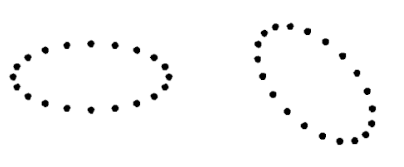
\includegraphics[width=0.5\textwidth]{figs/pol.png}
\caption{The plus(left) and cross(right)-polarizations of the gravitational waves.}
\end{figure}

The gravitational wave can have more polarizations (if we don't assume that the general relativity is correct), but this is not covered here.

\subsubsection{Waveform of Gravitational Waves}

Before two large objects (such as black holes) collide with each other, they have time to orbit. At this time, energy is released in the form of gravitational waves. Initially, low frequencies and low amplitude gravitational waves occur. And as the two objects continue to revolve and get closer to each other, their frequencies and amplitudes increase. Eventually, when the two objects approach a certain level or higher, the frequencies and amplitude increase dramatically.

Here is the waveform of the GW150914, which is the first detected gravitational-wave signal.

\begin{figure}[h]
\centering
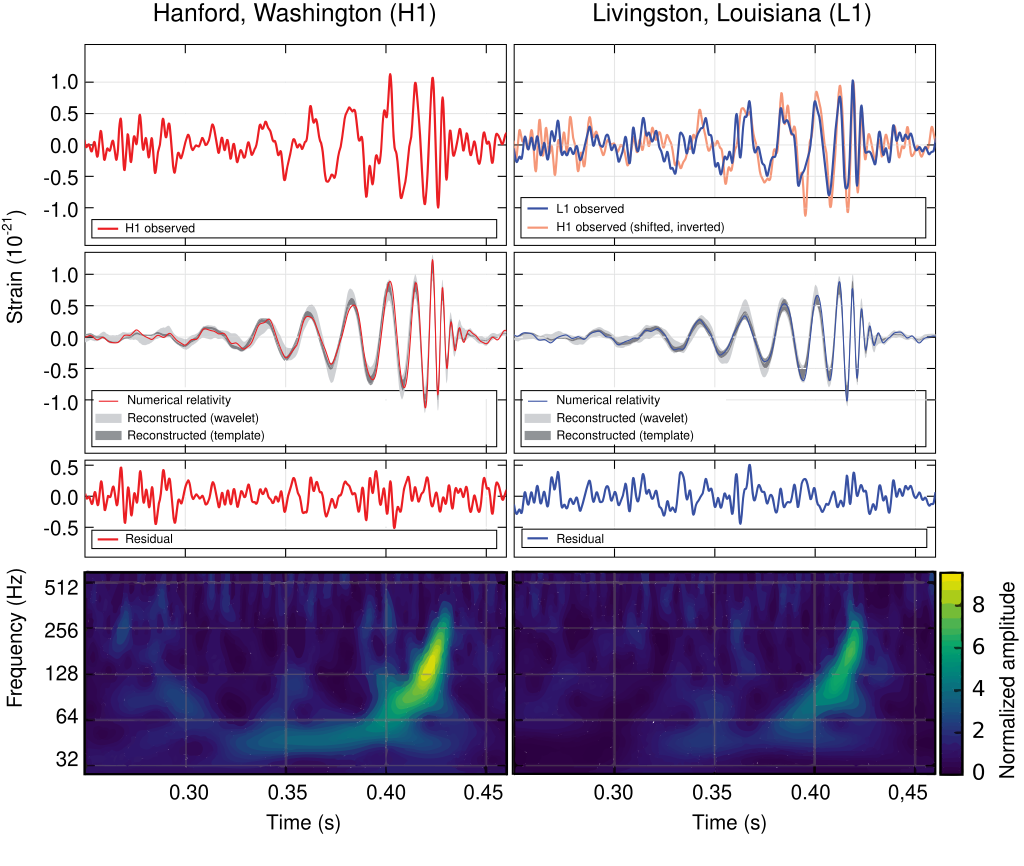
\includegraphics[width=0.7\textwidth]{figs/150914.png}
\caption{The waveform of GW150914. Figure from \href{https://en.wikipedia.org/wiki/First_observation_of_gravitational_waves}{Wikipedia: First Observation of Gravitational Waves}}
\end{figure}

Let's assume that two massive objects are orbiting each other in a circular orbit.

We define as $t_{\mathrm{ret}} = t - r/c$ (when the gravitational wave waveform we observe occurs) and $f$ as the frequency of the gravitational wave. $\theta$ is the angle between the observer and the straight line connecting the gravitational source and the axis of rotation of the gravitational source celestial body (the co-latitude) and $\phi$ is the phase.

And then we can estimate the waveform of the gravitational-wave.

\begin{align}
    h_+(t) &= \frac{4}{r} \left( \frac{G\mathcal{M}}{c^2} \right)^{\frac{5}{3}} \left( \frac{\pi f}{c} \right)^{\frac{2}{3}} \frac{1 + \cos^2{\theta}}{2} \cos{(2\pi f t_{\mathrm{ret}} + 2 \phi)} \\
    h_\times(t) &= \frac{4}{r} \left( \frac{G\mathcal{M}}{c^2} \right)^{\frac{5}{3}} \left( \frac{\pi f}{c} \right)^{\frac{2}{3}} \cos{\theta} \sin{(2\pi f t_{\mathrm{ret}} + 2 \phi)}
\end{align}

For more information such as the derivation of the formula, see \textit{Maggiore}(2008) Sec. 3 and 4.

\subsubsection{The Time to Coalescence}

About elliptical orbit, let's think that we have the samimajor axis $a_0$, the eccentricity $e_0$ and the orbital period $T_0$. The subscript $0$ means that they are initial value. And $M = m_1 + m_2$ is the total mass, $\mu$ is the reduced mass.

We can see the orbital period from the fact that the gravitational wave frequency $f$ is twice the orbital frequency.

We have the coalescence time $\tau_0$ as

\begin{align}
    \tau_0(a_0, e_0) &\simeq 9.829\mathrm{Myr} \left( \frac{T_0}{1\mathrm{hr}} \right)^{\frac{8}{3}} \left( \frac{M_\odot}{M} \right)^{\frac{2}{3}} \left( \frac{M_\odot}{\mu} \right) f(e_0) \\
    F(e_0) &= \frac{48}{19} \frac{1}{[g(e_0)]^4} \int_{0}^{e_0} de \ \frac{[g(e)]^4 (1 - e^2)^{5/2}}{e(1 + \frac{121}{304} e^2)} \simeq \frac{768}{429} (1 - e_0^{\ 2})^\frac{7}{2} \\
    g(e) &= \frac{e^{12/19}}{1 - e^2} \left( 1 + \frac{121}{304} e^2 \right)^\frac{870}{2299}
\end{align}

For circular orbit case, because eccentricity $e_0$ is 0, so the coalescence time $\tau_0$ is

\begin{equation}
    \tau_0 \simeq 9.829\mathrm{Myr} \left( \frac{T_0}{1\mathrm{hr}} \right)^{\frac{8}{3}} \left( \frac{M_\odot}{M} \right)^{\frac{2}{3}} \left( \frac{M_\odot}{\mu} \right)
\end{equation}

For more information such as the derivation of the formula, see \textit{Maggiore}(2008) from Sec. 4.1.1 to 4.1.3.

\subsubsection{Gravitational Lens}

\subsubsection{Signal}

The time-domain signal-strain-data we can see from the detector is expressed as a linear combination of $h_+$ and $h_\times$.

\begin{equation}
    h(t) = F_+(\hat{\mathbf{n}}) h_+(t) + F_\times (\hat{\mathbf{n}}) h_\times (t)
\end{equation}

Where $\hat{\mathbf{n}}$ is the direction vector. This is determined from polarization and azimuth. For more information, see \textit{Maggiore}(2008) Sec. 7.2.

The Python package Pycbc has a function of entering hplus, hcross, polarization, and azimuth to project it. For more information about this, see \href{https://pycbc.org/pycbc/latest/html/waveform.html}{Pycbc Waveform Documents}.

\subsubsection{Signal and Noise}

When detecting gravitational waves, the amplitude of noise is greater than that of ordinary signals. Therefore, it is necessary to identify the frequency characteristics of the signal in noise by Fourier transforming them.

[Physical part: formula]

\subsubsection{Detection Analysis}

\subsubsection{Interferometers}

\subsection{Statistical Methods}

\subsubsection{Bayes Theorem}

Given two probability distributions and conditional probabilities, the probability of two occurring simultaneously is as follows.

\begin{equation}
    P(A \cup B) = P(A|B) P(B) = P(B|A) P(A)
\end{equation}

Bayes' theorem is a way to find a conditional probability $P(B|A)$ when you know a conditional probability $P(A|B)$. The formula is as follows.

\begin{equation}
    P(B|A) = \frac{P(A|B)P(B)}{P(A)}
\end{equation}

The general formula is as follows.

\begin{equation}\label{mlm}
    P(x_0|A) = \frac{P(x_0) P(A|x_0)}{P(A)} = \frac{P(x_0) P(A|x_0)}{\int dx \ P(x) P(A|x)}
\end{equation}

For more information such as application example, visit \href{https://en.wikipedia.org/wiki/Bayes%27_theorem}{Wikipedia: Bayes Theorem}.

\subsubsection{Maximum Likelihood Method}

The likelihood is a probability known empirically beforehand. By formula(\ref{mlm}), we define the likelihood $\mathcal{L}$ as follows.

\begin{equation}
    \mathcal{L}(A|x) = P(x|A)
\end{equation}

Here, $A$ is the surrounding environment (parameters, such as the mass of the black holes, the distance from observer, etc.) that produces the result value, and $x$ is the result value. We know the result($x$) from observations, and we need to find the surrounding environment($A$) that produces the result.

Let the parameters such that the probability distribution $P(x|A)$ is maximized be called the estimated value $A_0$. In this case, we can estimate that the observation value $x$ is more likely to be generated by parameter $A_0$ compared to other parameters.

Therefore, when $x$ is fixed, we need to find $A$ so that the likelihood has an extreme value.

\begin{equation}
    A_0 = \underset{A}{\arg\max} \ {\mathcal{L}(A|x)}
\end{equation}

We can obtain parameters that derive the maximum likelihood in the preferred method of the two. (the latter is usually preferred here)

\begin{subequations}
    \begin{align}
        0 &= \frac{\partial{\mathcal{L}(A|x)}}{\partial A} \\
        0 &= \frac{\partial{\ln{\mathcal{L}(A|x)}}}{\partial A}
    \end{align}
\end{subequations}

For a thorough mathematical description or an explanation of an algorithm, etc., visit \href{https://en.wikipedia.org/wiki/Maximum_likelihood_estimation}{Wikipedia: Maximum Likelihood Estimation}.

\subsubsection{Metropolis-Hastings Method}

Markov Chain Monte Carlo(MCMC) method is an example of rejection method. In this method, we need a probability distribution(it is OK if not-renormalized).

Metropolis-Hastings method is one of the examples of MCMC. In this method, we need a probability distribution and a proposal distribution. Here I explain the algorithm only, not proof.\footnote{The notation and explanation are based on Okubo(2022), https://github.com/compsci-alliance/many-body-problems}\footnote{The proof is in Chib \& Greenberg(1995).}

The set of all states is $\{ \Gamma \}$. We have a probability distribution $P(\Gamma)$ and a proposal distribution $q(\Gamma | \Gamma')$,

Step 0: Prepare an initial state $\Gamma_0 \in \{ \Gamma \}$

\quad loop $t$

\qquad 1. Make next candidate state $\Gamma'$ randomly from the proposal distribution $q(\Gamma' | \Gamma_t)$

\qquad 2. Make a uniform random number $r \in [0,1]$

\qquad 3. Select the next state $\Gamma_{t + 1}$ based on $r$ as

\begin{equation}
    \Gamma_{t+1} = \begin{cases} \Gamma' & (r \leq a (\Gamma_t \to \Gamma') \\ \Gamma_t & (\mathrm{else}) \end{cases}
\end{equation}

Where the acceptance probability is as follows.

\begin{equation}
    a (\Gamma_t \to \Gamma') = \min{\left(1, \ \frac{P(\Gamma') q(\Gamma_t | \Gamma')}{P(\Gamma_t) q(\Gamma' | \Gamma_t)} \right)}
\end{equation}

The example problem is as follows.

\begin{example}

The probability density function is as follows.

\begin{equation}
    p(x) = 0.3 \frac{1}{2 \sqrt{2\pi}} \exp{\left(- \frac{(x + 5)^2}{8} \right)} + 0.7 \frac{1}{\sqrt{2\pi}} \exp{\left(- \frac{(x - 3)^2}{2} \right)}
\end{equation}

The proposal density funcion is a normal distribution function, as follows.

\begin{equation}
    q(x^* | x) = \frac{1}{10\sqrt{2\pi}} \exp{\left( -\frac{(x^* - x)^2}{200} \right)}
\end{equation}

Set initial state as random normal distribution with mean 0 and standard deviation 10. The probability density is as follows.

\begin{equation}
    p_0 (x_0) = \frac{1}{10\sqrt{2\pi}} \exp{\left( -\frac{x_0^{\ 2}}{200} \right)}
\end{equation}

Calculate the logarithm of the acceptance rate.

\begin{equation}
    \ln{a} = \ln{p(x^*)} - \ln{p(x_{t-1})} + \ln{q(x_{t-1} | x^*)} - \ln{q(x^* | x_{t-1})}
\end{equation}

Make a random $r$ from $(0,1]$ and compare $r$ and the acceptance rate.

\begin{align}
    \ln{\alpha} &= \min{(0, \ln{a})} \\
    \ln{r} \leq \ln{a} &\to x_{t} = x^* \\
    \ln{r} > \ln{a} &\to x_{t} = x_{t-1}
\end{align}

Repeat this 5000 times($t = 5000$).

The code is as follows.

\begin{python}[Python3]
import numpy as np
import math
import scipy.stats as stats
import matplotlib.pyplot as plt
def p(x):
    return 0.3 * (2 * math.sqrt(2 * math.pi)) ** (-1) * np.exp(-(x + 5) ** 2 / 8) + 0.7 * (math.sqrt(2 * math.pi)) ** (-1) * np.exp(-(x - 3) ** 2 / 2)
def logp(x):
    return np.log(p(x))
T = 5000
sigma = 10
for i in range(1, T+1):
    candidate = np.random.normal(size = 1, loc=learn[i-1], scale=sigma)
    loga = logp(candidate) - logp(learn[i-1]) + stats.norm(candidate, sigma).logpdf(learn[i-1]) - stats.norm(learn[i-1], sigma).logpdf(candidate)
    logalpha = min(0, loga)
    r = np.random.uniform(size=1)
    logr = math.log(r)
    if logr <= logalpha:
        learn = np.append(learn, candidate)
    else:
        learn = np.append(learn, learn[i-1])
grid = np.arange(-10, 10, 0.01)
plt.plot(grid, p(grid))
plt.hist(learn, bins = 40, density = True)
plt.show()
\end{python}

The result is as follows.

\begin{figure}[h]
\centering
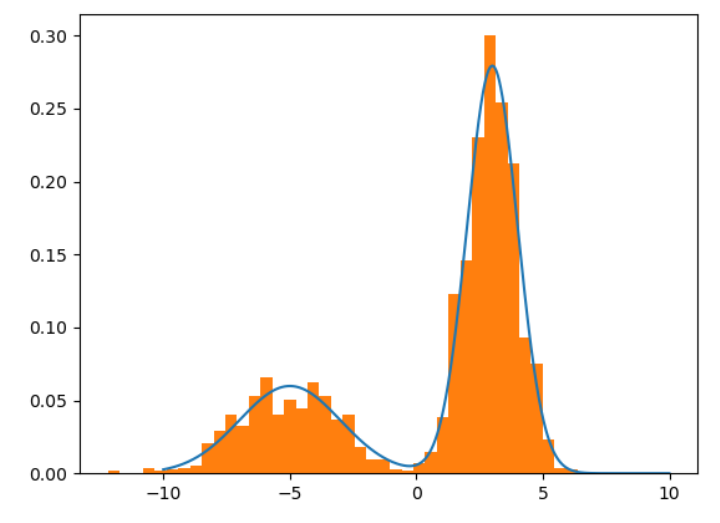
\includegraphics[width=0.5\textwidth]{figs/met.png}
\caption{Metropolis-Hastings example code result}
\end{figure}

\end{example}

This part deals with similar content as \href{https://en.wikipedia.org/wiki/Metropolis%E2%80%93Hastings_algorithm}{Wikipedia: Metropolis-Hastings Algorithm}, so you can read and compare them.

\subsubsection{Inverse Transform Method}

When we have a probability distribution $p(x)$, we can make a simulation program to generate that distribution.

The cumulative probability distribution $P(x)$ is as follows.

\begin{equation}
    P(x) = \int_{-\infty}^x p(x) \ dx
\end{equation}

Let's think about the slope of $P(x)$. This is a probability distribution $p(x)$.

\begin{align}
    y &\equiv P(x) \\
    dy &= p(x)dx
\end{align}

Therefore, we can know that $dy$ is proportional to the probability distribution. What that does mean?

Let us generate random numbers $y$ that have uniform distribution in the rages of $[0,1]$. If we choose a specific $y_0 \sim y_0 + dy$, we can get the number of $y$ such that $y_0 \leq y \leq y_0 + dy$. The number is proportional to $p(x)$.

\begin{equation}
    dy = p(x)dx \propto p(P^{-1}(y))
\end{equation}

Therefore, we can correspond y to x, as follows.

\begin{equation}
    x = P^{-1}(y)
\end{equation}

So the $x$ have the probability distribution $p(x)$.

I think the explanation might be difficult to understand, so let's see an example.

\begin{example}

The range of inclination angle in GWpy package is $-\pi/2 \leq \theta \leq \pi/2$, so if we want the isotropic spherical distribution, we should use cosine distribution rather than sine distribution. See equation (\ref{int}).

The distribution is as follows.

\begin{align}
    p(x) &= \begin{cases} \frac{1}{2} \cos{x} & ( -\pi/2 \leq x \leq \pi/2) \\ 0 & (\mathrm{else}) \end{cases} \\
    P(x) &= \begin{cases} 0 & (x \leq -\pi/2 ) \\ \frac{1}{2} \sin{x} + \frac{1}{2} & ( -\pi/2 \leq x \leq \pi/2) \\ 1 & (x \geq \pi/2 ) \end{cases} \\
    x &= P^{-1} (y) = \arcsin{(2y - 1)} \quad (0 \leq y \leq 1)
\end{align}

We will generate 10,000 number of random uniform numbers in $[0,1]$ and make cosine distribution. And for comparison, we will draw an exact cosine distribution function. The code is as follows.

\begin{python}[Python3]
import numpy as np
import matplotlib.pyplot as plt
a = []
for _ in range(10000):
    x = np.random.uniform(0,1)
    y = np.arcsin(2 * x - 1)
    a.append(y)
plt.hist(a, bins=100, density=True)
plt.plot(np.linspace(-np.pi/2, np.pi/2,100), 0.5*np.cos(np.linspace(-np.pi/2, np.pi/2,100)))
plt.show()
\end{python}

The result is as follows.

\begin{figure}[h]
\centering
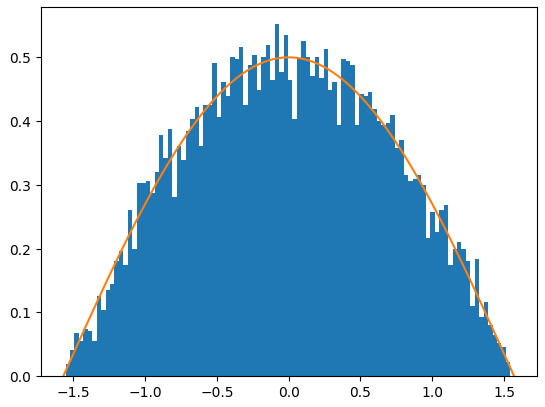
\includegraphics[width=0.5\textwidth]{figs/cos.png}
\caption{Code result and cosine distribution}\label{cosinedistribution}
\end{figure}

When making a prior set using bilby, we can use a cosine distribution provided in the package.

\begin{python}[Python3]
import numpy as np
import matplotlib.pyplot as plt
import bilby
priors = bilby.core.prior.PriorDict()
priors['dec'] = bilby.core.prior.Cosine(name = 'dec')
samples = priors.sample(10000)
plt.hist(samples['dec'], bins=100, density=True)
plt.plot(np.linspace(-np.pi/2, np.pi/2,100), 
         0.5*np.cos(np.linspace(-np.pi/2, np.pi/2,100)))
plt.show()
\end{python}

The result is almost same as Figure \ref{cosinedistribution}.

\end{example}

For more information, visit \href{https://en.wikipedia.org/wiki/Inverse_transform_sampling}{Wikipedia: Inverse Transform Sampling}.

\subsubsection{Confusion Matrix and ROC Curve}

The confusion matrix is used to evaluate the performance of the algorithm. It can be expressed as follows.

\begin{table}[h]
    \centering
    \begin{tabular}{c|cc}
         & Prediction: Positive & Prediction: Negative \\ \hline
        Actual result: Positive & True Positive (TP) & False Negative (FN)\\
        Actual result: Negative & False Positive (FP) & True Negative (TN)
    \end{tabular}
    \caption{Confusion Matrix}
    \label{confusion}
\end{table}

False positive rate(False alarm rate) is the proportion of data predicted as positive among data that are actually negative.

\begin{equation}
    \text{False positive rate} = \frac{\text{FP}}{\text{FP} + \text{TN}}
\end{equation}

Sensitivity(True positive rate) is the proportion of data that is actually positive, and the prediction result is also positive.

\begin{equation}
    \text{Sensitivity} = \frac{\text{TP}}{\text{TP} + \text{FN}}
\end{equation}

We can get the likelihood, accuracy, etc.. For more information about those, visit \href{https://en.wikipedia.org/wiki/Confusion_matrix}{Wikipedia - Confusion Matrix}.

Receive Operating Characteristic(ROC) curve is a plot that illustrates the performance of a binary classifier model at varying threshold values. The horizontal axis of the ROC curve is false positive rate, and the vertical axis is sensitivity.

The comparison curve is the $y=x$ straight line, which means that if the ROC curve is above $y=x$, the judgment was more correctly made than complete random classification, and if it is below, the classification was worse than complete random classification. For more information about those, visit \href{https://en.wikipedia.org/wiki/Receiver_operating_characteristic}{Wikipedia - Receive Operating Characteristic}.

\begin{figure}[h]
\centering
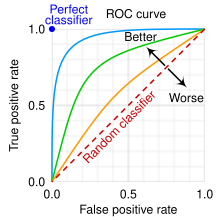
\includegraphics[width=0.5\textwidth]{figs/roc.png}
\caption{ROC curve - by Wikipedia}\label{roc}
\end{figure}

\section{Data Analysis Tutorial}

GWOSC Tutorial: Optional.\footnote{You can do \href{https://gw-odw.thinkific.com/courses/odw2024}{GWOSC TUTORIAL 2024}: tutorial 1.1-3.3 first. But this tutorial referred to GWOSC tutorial much, so I recommend doing one and reading another as a dictionary.}

\subsection{Tutorial 1}

\subsubsection{Tutorial 1.1 - View Data with GWOSC Package}

With 'gwosc' pacakge, you can

1. Know what event are in a (particular) catalog: for example, you can know GW150914, GW151012,... are in GWTC-1(confident) event catalog.

2. Find gravitational-wave datasets for a specific time

3. Know the event time(GPS) of the gravitational-wave detection

4. Get the URLs of a specific gravitational-wave event data

5. Filter data satisfying certain parameters

etc..

For more understanding, you can visit \href{https://gwosc.readthedocs.io/en/stable/index.html}{GWOSC 0.7.1 documentation}.

\subsubsection{Tutorial 1.2 - Fetch Timeseries}

'gwpy', 'pycbc', 'bilby' are Python packages which is used to analyse gravitational-wave data.

Depending on the analyzing method, there are cases in which data formatted by a specific package should be used. For a few sections from here you learn:

How to open and plot the data,

How to convert the timeseries-data into a frequencyseries-data,

How to generate and inject signal data,

How to change the format so that the data to be compatible with each other,

etc..

In this section, you fetch open-data(timeseries data) with 'gwpy', 'pycbc' and 'bilby' package.

\

1. GWpy\footnote{https://gwpy.github.io/docs/stable/overview/}

Prepare the environment.\footnote{It will be explained next time, please distinguish it from PyCBC TimeSeries.}

\begin{python}[Python3]
import warnings
warnings.filterwarnings("ignore", "Wswiglal-redir-stdio")
import gwpy
from gwpy.timeseries import TimeSeries
\end{python}

Fetching open-data, we need to

1. Know the event time(GPS).

2. Choose the interferometer.

At first, we use GWOSC package to know the GPS time. In this step, we fetch GPS time and set the segment time(for this example, GPS segment to 10 seconds around GPS time).

You can print gps and segment for check also.

\begin{python}[python3]
import gwosc
from gwosc.datasets import event_gps

gps = event_gps('GW190412')
segment = (int(gps)-5, int(gps)+5)
\end{python}

And then, we need to download open data from interferometer data.

The interferometers we can use in GWOSC package are as follows.

'L1': LIGO-Livingston

'H1': LIGO-Handford

'G1': GEO-600

'V1': (Advanced) Virgo

'K1': KAGRA

Using TimeSeries (from gwpy.timeseries), we can fetch the data.

\begin{python}[python3]
    FetchedData = TimeSeries.fetch_open_data('L1', *segment, verbose = True)
\end{python}

You can plot easily using GWOSC TimeSeries.

\begin{python}[python3]
    plot = FetchedData.plot()
    plot.show() # If you can't see the plot by previous line, run this line also.
\end{python}

2. PyCBC

In PyCBC, we don't need to know GPS time exactly.(So we don't need GWOSC.)

We can use interferometers in PyCBC almost same as in GWpy.

\begin{python}[python3]
    import pycbc
    from pycbc.catalog import Merger
    import matplotlib.pyplot as plt

    merger = Merger("GW150914")
    strain = merger.strain('H1')
    plt.plot(strain.sample_times, strain)
    plt.show()
\end{python}

The default sampling time is 1/4096 second, and we will learn downsampling and removing low-frequence in the next section.

\ 

3. bilby

In bilby, we need to fetch data from GWpy.

\begin{python}[python3]
    import bilby
    import gwosc
    from gwosc.datasets import event_gps
    import gwpy
    from gwpy.timeseries import TimeSeries

    #Using GWpy, download the gravitional-wave data.
    gps = event_gps('GW150914')
    Data = TimeSeries.fetch_open_data('L1', gps - 2, gps + 2, sample_rate = 4096, cache = True)

    #Set interferometer and strain data using bilby
    L1 = bilby.gw.detector.get_empty_interferometer('L1')
    L1.set_strain_data_from_gwpy_timeseries(Data)
\end{python}

\subsubsection{Tutorial 1.3 - Generate a Signal Timeseries}

With PyCBC, we can generate a signal. In this example, using the approximant 'IMRPhenomD', we generate a binary-black-holes signal.

\begin{python}[python3]
    from pycbc.waveform import get_td_waveform
    sampling_rate = 4096
    hp, hc = get_td_waveform(approximant = 'IMRPhenomD',
                             mass1 = 36,
                             mass2 = 29,
                             delta_t = 1 / sampling_rate,
                             f_lower = 20,
                             distance = 410)
\end{python}

You can use other approximants (for example TaylorT4 for binary-neutron-stars) or add other parameters (for example spins). See \href{https://pycbc.org/pycbc/latest/html/pycbc.waveform.html#pycbc.waveform.waveform.get_td_waveform}{here}.

\subsubsection{Tutorial 1.4 - Resample Timeseries Data}

1. GWpy

From tutorial 1.2, we have fetched data named FetchedData.

First, let's check sampling rate and delta t(the inverse of the sampling rate).

\begin{python}[python3]
    print(FetchedData.sample_rate)
    print(FetchedData.dt)
\end{python}

We can resample(downsample) the data easily.

\begin{python}[python3]
    ResampledData = FetchedData.resample(1024)
    print(ResampledData.sample_rate)
    print(ResampledData.dt)
\end{python}

2. PyCBC

From tutorial 1.2, we have fetched data named strain.

First, let's check sampling rate and delta t.

\begin{python}[python3]
    print(strain.sample_rate)
    print(strain.delta_t) #not dt
\end{python}

We can resample(downsample) the data with 'resample\_to\_delta\_t'.

\begin{python}[python3]
    from pycbc.filter import resample_to_delta_t

    resampled = resample_to_delta_t(strain, 1/1024)
    print(resampled.sample_rate)
    print(resampled.delta_t)
\end{python}

\subsubsection{Tutorial 1.5 - Resize a TimeSeries}

With PyCBC, we can resize the PyCBC timeseries. 

1. Time Slice

(0,4) means that we only have time from 0 to 4 seconds left in these timeseries.

\begin{python}[python3]
    import pycbc
    from pycbc.waveform import get_td_waveform
    hp, hc = get_td_waveform(approximant = "IMRPhenomD",
                             mass1 = 36,
                             mass2 = 29,
                             delta_t = 1 / sampling_rate,
                             f_lower = 20,
                             distance = 410)
    hp.start_time = hp.start_time + 2
    hc.start_time = hc.start_time + 2
    hpslice = hp.time_slice(0,4)
    hcslice = hc.time_slice(0,4)
\end{python}

2. Crop

(0.5,0.5) means that we throw away the first 0.5 seconds and the last 0.5 seconds in these timeseries.

\begin{python}[python3]
    import pycbc
    from pycbc.waveform import get_td_waveform
    hp, hc = get_td_waveform(approximant = "IMRPhenomD",
                             mass1 = 36,
                             mass2 = 29,
                             delta_t = 1 / sampling_rate,
                             f_lower = 20,
                             distance = 410)
    hp.start_time = hp.start_time + 2
    hc.start_time = hc.start_time + 2
    hpcrop = hp.crop(0.5,0.5)
    hccrop = hc.crop(0.5,0.5)
\end{python}

3. Resize

(65536) means that we resize the data, length to 65536. The length is (duration time)$\times$(time interval). Here, 'resize' adjusts the length by adding a sample before or after the data if necessary.

\begin{python}[python3]
    import pycbc
    from pycbc.waveform import get_td_waveform
    hp, hc = get_td_waveform(approximant = "IMRPhenomD",
                             mass1 = 36,
                             mass2 = 29,
                             delta_t = 1 / sampling_rate,
                             f_lower = 20,
                             distance = 410)
    hp.start_time = hp.start_time + 2
    hc.start_time = hc.start_time + 2
    hpcrop = hp.resize(65536)
    hccrop = hc.resize(65536)
\end{python}

\subsubsection{Tutorial 1.6 - Generate FrequencySeries Data}

With PyCBC, we can generate a Frequencyseries data. The method is similar to the Timeseries part. The return is a frequency domain gravitational waveform.

\begin{python}[python3]
    from pycbc.waveform import get_fd_waveform
    hp, hc = get_td_waveform(approximant = 'IMRPhenomD',
                             mass1 = 36,
                             mass2 = 29,
                             delta_f = 0.25,
                             f_lower = 20,
                             distance = 410)
\end{python}

For more information, see \href{https://pycbc.org/pycbc/latest/html/pycbc.waveform.html#pycbc.waveform.waveform.get_td_waveform}{PyCBC Document: Waveform}

\subsubsection{Tutorial 1.7 - Change Format}

We can change data format, for example, PyCBC to GWpy, etc..

We will change a PyCBC timeseries to GWpy timeseries. The basic method is to copy and paste the numbers of time data and the corresponding time series data, so it is easy to convert to the format not introduced here. Try it yourself.

Example material: PyCBC timeseries(named 'sample', time interval: 1/4096 s, start time: 0 s)

\begin{python}[python3]
    import pycbc
    from pycbc.types import TimeSeries
    import gwpy
    from gwpy.timeseries import TimeSeries as GWTimeSeries
    GWsample = GWTimeSeries(
    sample,
    dt = 1/4096,
    t0 = 0)
\end{python}

\subsection{Tutorial 2}

\subsubsection{Tutorial 2.1 - Generate a White Gaussian Noise}

When generating a white gaussian noise, the PSD must be flat.

You can generate the PSD with bilby and generate a white gaussian noise. In this example, we make a flat PSD whose frequency range is from 0 to 2048Hz and frequency interval is 0.25Hz

\begin{python}[python3]
    import numpy as np
    import bilby
    freq = np.linspace(0,2048,8193)
    psd = 8193 * [1. * 1e-40]
    Ifo = bilby.gw.detector.get_empty_interferometer('K1')
    Ifo.power_spectral_density = bilby.gw.detector.PowerSpectralDensity(
        frequency_array = freq,
        psd_array = psd)
\end{python}

Let's make a white gaussian noise from the flat PSD we made.

\begin{python}[python3]
    Ifo.set_strain_data_from_power_spectral_density(
        sampling_frequency=4096,
        duration=4096,
        start_time=0)
\end{python}

You can check if this noise is gaussian.

\begin{python}[python3]
    plt.hist(Ifo.strain_data.time_domain_strain, bins = 100)
    plt.show()
\end{python}

You can check if this noise is white.

\begin{python}[python3]
    plt.loglog(Ifo.strain_data.frequency_array, abs(Ifo.strain_data.frequency_domain_strain))
    plt.show()
\end{python}

\subsubsection{Tutorial 2.2 - Fetch PSD and Generate Coloured Noise}

With bilby package, you can generate a coloured PSD for simulation. Each of the interferometers in the bilby package has its own PSD by default.

\begin{python}[python3]
    import bilby
    Ifo = bilby.gw.detector.get_empty_interferometer('K1')
    Ifo.set_strain_data_from_power_spectral_density(
        sampling_frequency=4096,
        duration=4096,
        start_time=0)
\end{python}

We fetched KAGRA simulation PSD and set strain data from the PSD. You can choose 'L1', 'H1' or 'V1', etc for other interferometers.

You can see the PSD.

\begin{python}[python3]
    import matplotlib.plot as plt
    plt.loglog(Ifo.power_spectral_density.frequency_array, Ifo.power_spectral_density.psd_array)
    plt.show()
\end{python}

You can check if this noise is gaussian.

\begin{python}[python3]
    plt.hist(Ifo.strain_data.time_domain_strain, bins = 100)
    plt.show()
\end{python}

You can check if this noise is coloured.

\begin{python}[python3]
    plt.loglog(Ifo.strain_data.frequency_array, abs(Ifo.strain_data.frequency_domain_strain))
    plt.show()
\end{python}

You can plot the noise timeseries.

\begin{python}[python3]
    plt.plot(Ifo.strain_data.time_array, Ifo.strain_data.time_domain_strain)
    plt.show()
\end{python}

\subsubsection{Tutorial 2.3 - Inject a Signal to the Noise}

We generated a noise and signal. To inject, the two timeseries must be compatible (have the same format), and the time interval and duration of the two must be the same.

If the signal's format is GWPy(I recommend), then convert the bilby noise to GWPy timeseries and inject. PyCBC is also recommended, and the method is almost same. See \href{https://pycbc.org/pycbc/latest/html/modules.html}{PyCBC Document} and \href{https://gwpy.github.io/docs/stable/}{GWPy Document}.

1. GWPy

\begin{python}[python3]
    from gwpy.timeseries import TimeSeries
    Ifo.set_strain_data_from_power_spectral_density(
        sampling_frequency=4096,
        duration=4,
        start_time=0)
    Noise = TimeSeries(
        Ifo.strain_data.time_domain_strain,
        dt = 1/4096,
        t0 = 0)
\end{python}

2. bilby

We can inject a signal to the noise, using bilby. I only put it here for the reference that there is an example of this. See \href{https://lscsoft.docs.ligo.org/bilby/api/bilby.gw.detector.inject_signal_into_gwpy_timeseries.html}{bilby Document} for more information.

\subsection{Tutorial 3}

\subsubsection{Tutorial 3.1 - Q Transforms}

We can do Q-transform with GWpy. For more informations such as basic knowledge, visit \href{https://iopscience.iop.org/article/10.1088/0264-9381/21/20/024}{this article}.

Material: GWpy timeseries (named 'data')

\begin{python}[python3]
    import warnings
    warnings.filterwarnings("ignore", "Wswiglal-redir-stdio")
    import gwpy
    import matplotlib.pyplot as plt

    qt = data.q_transform(frange=(30, 500))
    plot = qt.plot()
    plot.colorbar(label="Normalised energy")
\end{python}

We can set colorbar range also. This helps to see signals hidden in loud noise (e.g., shot noise, etc.).

\begin{python}
    plot.colorbars[0].mappable.set_clim(0,20)
    plot.refresh()
    plot
\end{python}

\subsubsection{Tutorial 3.2 - Matched Filtering Test}

We use PyCBC.

Material. The formats should be PyCBC timeseries.

1. PSD

2. Strain data (ex. noise of the detector, fetched strain data, or signal injected to the noise, etc)

If you generate noise strain data, please use the PSD data. If you fetch strain data, please make(estimate) the PSD from the strain data fetched. The sampling frequency interval has to be same between PSD and the strain data.

3. Sample waveform data (hplus timeseries)

The sampling time interval of the sample has to be same as that of the strain data.

Let's assume that we have the strain data(named 'strain'), PSD data(named 'psd'), and the sample waveform data(named 'hp').

First, match the length of hp and sample.

\begin{python}[python3]
    import numpy as np
    import pycbc
    from pycbc.waveform import get_td_waveform
    from pycbc.filter import matched_filter
    hp.resize(len(sample))
\end{python}

The time of the strain data has to be different from that of the sample. If you generated the noise data, please do this work. (If you fetched strain data, this work is not necessary.)

\begin{python}[python3]
    hp.start_time = hp.start_time - (len(sample) * hp.delta_t + 1)
\end{python}

Do matched filtering. We should remove time corrupted by the template filter and the psd filter. We assume that the time-length of the sample is long enough, so 2e set the cropping time to the first 4 seconds and the last 4 seconds. (This time can change fluidly of course.)

\begin{python}
    snr = matched_filter(hp,
                         sample,
                         psd=psd,
                         low_frequency_cutoff=20)
    snr = snr.crop(4, 4)
    peak = abs(snr).numpy().argmax()
    snrp = noisesnr[peak]
    snrp = abs(snrp)
    time = snr.sample_times[peak]
    print(time)
    print(snrp)
\end{python}

\subsubsection{Tutorial 3.3 - Parameter Estimating}

Using bilby, we can estimate the parameter(The source of the gravitational-wave).

Material

1. Strain data

You can fetch the strain data, or use generated noise data or signal injected to noise.

2. Waveform Arguments (bilby)

3. Prior (bilby)

First, set prior. Bilby runs Monte Carlo process or Dynesty process to estimate the parameters. In this example, we will estimate the GW150914 parameters.

\begin{python}[python3]
    import bilby
    from bilby.core.prior import Uniform, PowerLaw
    prior = bilby.core.prior.PriorDict()
    prior['chirp_mass'] = Uniform(name = 'chirp_mass',
                                  minimum = 26.0,
                                  maximum = 30.0)
    prior['mass_ratio'] = Uniform(name = 'mass_ratio',
                                  minimum = 0.5,
                                  maximum = 1)
    prior['phase'] = Uniform(name = 'phase',
                             minimum = 0,
                             maximum = 2 * np.pi)
    prior['geocent_time'] = Uniform(name = 'geocent_time',
                                    minimum = 2 - 0.1,
                                    maximum = 2 + 0.1)
    prior['a_1'] = 0.0
    prior['a_2'] = 0.0
    prior['luminosity_distance'] = PowerLaw(alpha = 2,
                                            name = 'luminosity_distance',
                                            minimum = 50,
                                            maximum = 2000,
                                            unit = 'Mpc',
                                            latex_label = '$d_L$')
\end{python}

\subsubsection{Tutorial 3.4 - Visualing the Results}

\subsection{Tutorial 4}
\subsubsection{Turotial 4.1 - Loop, Parallel Processing}

Using 'argparse' package, we can do parallel processing.

We set variables and make a program that prints the number.

\begin{python}[python3]
    import argparse
    import multiprocessing
    from multiprocessing import Pool
    parser = argparse.ArgumentParser(
        prog = 'ProgramName',
        description = 'What the program does',
        epilog = 'Text at the bottom of help')
    parser.add_argument('-c',
                        '--count',
                        type=int,
                        default=1,
                        help='The number of simulation times')
    parser.add_argument('-p',
                    '--process',
                    type=int,
                    default=1,
                    help='The number of processes for multi-processing')
    args = parser.parse_args()
    def run(n):
        print(n+1)
    pool = Pool(args.process)
    inputs = range(args.count)
    pool.map(run, inputs)
\end{python}

In bash, we will run this program running 20 steps with 4 processes. (The file name is test.py for example.)

\begin{verbatim}
    $ python3.10 test.py -c 10 -p 4
\end{verbatim}

The result will be mixed number, not the order of 1,2,3,... .

This is because 20 tasks are divided and executed by 4 processes. If we set '-p 1', the result will be the order of 1,2,3,... .

We cannot do bilby multi-processing by this method. Instead, multiprocessing is done inside the bilby package. In tutorial 3.3(parameter estimation), we set run\_sampler as follows.

\begin{python}[python3]
    result_short = bilby.run_sampler(
            likelihood,
            prior,
            sampler = 'dynesty',
            outdir = 'short',
            label = 'GW150914',
            conversion_function = bilby.gw.conversion.generate_all_bbh_parameters,
            nlive = 250,
            dlogz = 1.,
            clean = True,
            npool = args.process)
\end{python}

Then bilby will send message that we will multitask with (the set number of) processes.

\subsubsection{Tutorial 4.2 - Saving and Reading CSV Files}

After the iterative work, we can store the collected data. In this part, we will save the data as csv format.

\begin{python}[python3]
    import csv
    result = []
    def run(n):
        result.append(n)
    for n in range(30):
        run(n)
    with open('result.csv',
          'w',
          newline = '') as saveresult:
    csv.writer(saveresult).writerow(result)
\end{python}

Also, we can read a csv file.

\begin{python}[python3]
    data = 'result.csv'
    output = []
    with open(data,
              'r',
              newline = '') as f:
        reader = csv.reader(f)
        for row in reader:
            output.append(row)
    print(output)
\end{python}

\subsubsection{Tutorial 4.3 - Drawing ROC Curve}

The ROC curve is the plot of the true positive rate (TPR) against the false positive rate (FPR) at each threshold setting. For more information, visit \href{https://en.wikipedia.org/wiki/Receiver_operating_characteristic}{Wikipedia page}.

The higher the lower area of the curve, the better this data is classified.

Let's say we have positive and negative data separately(Named PositiveData and NegativeData as python lists). The data value at this time should be a real number.

\begin{python}[python3]
    import numpy as np
    import sklearn
    from sklearn.metrics import roc_curve, auc
    from sklearn.model_selection import train_test_split
    print(len(PositiveData))
    print(len(NegativeData))
\end{python}

Let's give positive data '1' and negative data '0', and do an analysis.

\begin{python}[python3]
    DataTrue = [0] * len(NegativeData) + [1] * len(PositiveData)
    Scores = NegativeData + PositiveData
    fpr, tpr, thresholds = roc_curve(DataTrue, Scores)
\end{python}

We can plot the ROC curve.

\begin{python}[python3]
    import matplotlib.pyplot as plt
    plt.plot(fpr, tpr)
    plt.legend(loc = 2)
    plt.xlabel('Flase Alarm Probability')
    plt.ylabel('Detection Probability')
    plt.title('ROC Curve')
    plt.show()
\end{python}

For more information, visit \href{https://scikit-learn.org/dev/modules/generated/sklearn.metrics.roc_curve.html}{Scikit-learn homepage}.

\section{TESLA based on GstLAL}
\subsection{Connecting to a LIGO Data Grid}
\subsubsection{How to Add a SSH Key}

When you are using TESLA, it's very convenient to connect to LIGO Data Grid.

This guide follows \href{https://computing.docs.ligo.org/guide/computing-centres/ldg/}{the LIGO Computing Guide}.

Because we are KAGRA member, please enter \href{https://registry.gw-astronomy.org/}{GW-Astronomy Registry}.\footnote{The link for offline(paper-book) users: https://registry.gw-astronomy.org/}

Click 'Services' on the left and click 'Click to Request' of 'LDG Account Request' among the main items.

\begin{figure}[h]
\centering
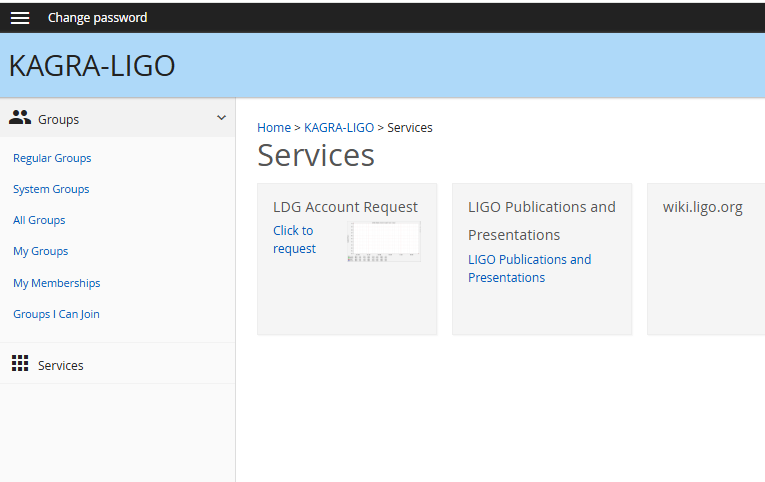
\includegraphics[width=0.6\textwidth]{figs/profile.png}
\caption{Add a SSH key}
\end{figure}

Affiliation has to be selected as 'Student', and the purpose of the current study has to be roughly written in the Justification. And click 'SUBMIT'.

Read the authorize form and aggree, and go to the next step.

And then click 'Authenticators'. Then you can see 'Add LDG SSH key' page, and in that page, you can add your SSH PUBLIC key. If you don't have an SSH key, see section \ref{SSH}.

\subsubsection{Login to the LIGO Data Grid}

If you uploaded the SSH key, you can enter to the LIGO Data Grid(the remote computer). It may take some time for the SSH key to be uploaded and logged in.

You can see the login hosts of \href{https://computing.docs.ligo.org/guide/computing-centres/hawk/}{Hawk}, \href{https://computing.docs.ligo.org/guide/computing-centres/cit/}{Caltech}, \href{https://computing.docs.ligo.org/guide/computing-centres/iucaa/}{IUCAA}, \href{https://computing.docs.ligo.org/guide/computing-centres/lho/}{LIGO-Hanford}, \href{https://computing.docs.ligo.org/guide/computing-centres/llo/}{LIGO-Livingston}, \href{https://computing.docs.ligo.org/guide/computing-centres/nemo/}{Nemo(UWM)} or \href{https://computing.docs.ligo.org/guide/computing-centres/psu/}{Gwave(PSU)}. I usually login to Caltech host.

\begin{verbatim}
    $ ssh seonjun.kwon@ldas-pcdev2.ligo.caltech.edu
\end{verbatim}

\subsection{Install the TESLA}

You can use GstLAL in LIGO Grid, or another supercomputer(for example, RESCEUBBC).

This guide was written with the help of Dr. Alvin Li.

\subsubsection{Use TESLA in the LIGO Grid}

Login to LIGO Grid and make a directory.

\begin{verbatim}
    $ mkdir Lensing
    $ cd Lensing
\end{verbatim}

There is a package in Dr. Alvin Li's directory that he has organized for download in batches.

\textbf{Use the Environment Directly: Recommended}

I recommend to use Dr Alvin Li's virtual environment directly, because Dr. Alvin Li can upgrade the elements of the TESLA environment, and in that case, it's very annoying to copy the new environment (upgrade the environment).

Set the nickname of the directory. For example, 'lensingenv'.

Vim into the '.bashrc' file.

\begin{verbatim}
    $ vi ~/.bashrc
\end{verbatim}

Add a phrase as below,

\begin{verbatim}
    export lensingenv=home/alvin.li/.conda/envs/tesla_o4a_analysis_240331/
\end{verbatim}

And reload the bashrc file.

\begin{verbatim}
    $ source ~/.bashrc
\end{verbatim}

The setup is over, so you don't have to modify or reload the '.bashrc' file as above from next time, even if you start the session anew.

You can load a virtual environment right away.

\begin{verbatim}
    $ conda activate $lensingenv
\end{verbatim}

\textbf{Install the Environment: NOT Recommended}

Let's create a Conda virtual environment by copying it.

\begin{verbatim}
    $ conda create --name testlensing --clone \
        /home/alvin.li/.conda/envs/tesla_o4a_analysis_240331
\end{verbatim}

This is the end of the installation.

The name of the package should not overlap. For example, if you set it to igwn-py39, you get an error that the name overlaps.

\subsubsection{Use TESLA in Another Supercomputer}

Basically, you can follow \href{https://git.ligo.org/alvin.li/tesla/-/tree/o4a_version_1.0}{Dr. Alvin Li's TESLA guide} in its entirety. It has been approved that it is okay to copy-paste all of this guide, and parts that are not in the guide will also be described here.

\textbf{SSH Login}

You need permission to connect to LIGO GIT on that supercomputer. Let's create an SSH key in the Ed25519 format from the home directory.

\begin{verbatim}
    $ ssh-keygen -t ed25519
    $ cd .ssh
    $ vi id_ed25519.pub
\end{verbatim}

Go to the \href{https://git.ligo.org/-/user_settings/ssh_keys}{SSH key page} of the User Settings page of the LIGO GIT.(You need to login to the LIGO GIT.) And click 'Add new key' button.

Copy and paste the entire contents of your 'ed\_25519.pub' file into the 'key' column. And click 'Add key'. Then you will get permission to clone the package files.

\textbf{Conda Environment}

You will need to first create a working python3 conda environment. We have a suggested conda YAML file included in this git repo tesla\_conda.yaml. Download the conda yml file via

\begin{verbatim}
    $ mkdir lensingenv
    $ cd lensingenv
    $ git archive --remote=git@git.ligo.org:alvin.li/tesla.git
        o4a_version_1.0 tesla_conda.yaml | tar -x
\end{verbatim}

Vim into tesla\_conda.yaml. In the last line, modify name: igwn-py39 to the name of the conda environment you want, for example, tesla\_o4a\_py39\_231228.

Of course, you don't need to vim that file and change the environment name, if you don't have 'igwn-py39' already.

Enter below.

\begin{verbatim}
    $ conda env create --file tesla_conda.yaml
\end{verbatim}

Activate the environment.

\begin{verbatim}
    $ conda activate igwn-py39
\end{verbatim}

\textbf{python-ligo-lw}

From now on, proceed with the igwn-py39 virtual environment in operation. (If not activate, enter below.)

\begin{verbatim}
    $ conda activate igwn-py39
\end{verbatim}

Because the cluster's ligolw is not up to date (especially for ligolw\_sqlite), we will need to install our own version of ligolw. To do so, first go to the conda environment directory that you have built.

For example, you can check the directory with

\begin{verbatim}
    $ vi ~/.conda/environments.txt
\end{verbatim}

And go into the directory that says igwn-py39 is in this text file. For example, (The directory may vary depending on the person or environment.)

\begin{verbatim}
    $ cd ~/anaconda3/envs/igwn-py39
\end{verbatim}

Make a new directory via mkdir src and change directory into it via cd src. Then clone the \href{https://git.ligo.org/kipp/python-ligo-lw/-/tree/1.8.x?ref_type=heads}{python-ligo-lw git repository}. (Note that -b 1.8.x is essential.)

\begin{verbatim}
    $ mkdir src
    $ cd src
    $ git clone git@git.ligo.org:kipp.cannon/python-ligo-lw.git -b 1.8.x
\end{verbatim}

And then change directory, and install the python package.

\begin{verbatim}
    $ cd python-ligo-lw
    $ pip3 install . --prefix ~/anaconda3/envs/igwn-py39/
\end{verbatim}

\textbf{doxygen}

To install doxygen, simply run

\begin{verbatim}
    $ conda install -c conda-forge doxygen
\end{verbatim}

\textbf{Boost Library}

For some reason, the Boost library on the clusters are deprecated. You will have to update it manually by running

\begin{verbatim}
    $ conda install boost boost-cpp libboost libboost-devel libboost-headers
        libboost-python libboost-python-devel
\end{verbatim}

\textbf{GstLAL}

We will be using the O3 version of GstLAL. First, go to the src directory in your conda environment.

\begin{verbatim}
    $ cd ~/anaconda3/envs/igwn-py39/src
\end{verbatim}

Clone the gstlal git repository. (Note that the -b mcvt\_plus\_fastpath\_updated is important.)

\begin{verbatim}
    $ git clone git@git.ligo.org:lscsoft/gstlal.git -b mcvt_plus_fastpath_updated
\end{verbatim}

Change directory into gstlal.

\begin{verbatim}
    $ cd gstlal
\end{verbatim}

Then run the following command to install gstlal.(./00init.sh to -j 8; \ is the same line.) If you are confused, copy the contents of \href{https://git.ligo.org/alvin.li/tesla/-/tree/o4a_version_1.0}{the guide} and modify only the 'path to conda environment' part to your conda environment location, and paste it.

\begin{verbatim}
    $ folders=(gstlal gstlal-ugly gstlal-calibration gstlal-burst gstlal-inspiral)
      path_to_conda_environment=~/anaconda3/envs/igwn-py39/
      for folder in "${folders[@]}" ; do \
	      echo ${folder} ; \
	      cd ${folder} ; \
	      ./00init.sh ; ./00init.sh && ./configure --prefix=${path_to_conda_environment}
              --with-zlib=$CONDA_PREFIX && make -j 8 && make install -j 8 ; \
	      cd ../ ; \
      done
\end{verbatim}

\textbf{gwpopprior}

Gwpopprior is used to create a targeted population model for the targeted search.

Go to the src directory in your conda environment.

\begin{verbatim}
    $ cd ~/anaconda3/envs/igwn-py39/src
\end{verbatim}

Clone the numerical-mass-model git repository. (Note that the -b o4a\_tesla\_version\_1.0 is important.)

\begin{verbatim}
    $ git clone git@git.ligo.org:heather-fong/numerical-mass-model.git -b
        o4a_tesla_version_1.0
\end{verbatim}

Change directory into numerical-mass-model.

\begin{verbatim}
    $ cd numerical-mass-model
\end{verbatim}

Then install gwpopprior via

\begin{verbatim}
    pip3 install . --prefix ~/anaconda3/envs/igwn-py39/
\end{verbatim}

\textbf{configobj}

You will also need to install configobj. To do so, run the following command. (This can be done in any directory.)

\begin{verbatim}
    $ pip3 install configobj --prefix ~/anaconda3/envs/igwn-py39/
\end{verbatim}

\textbf{numexpr}

If you use the igwn-py39.yml file to set up the conda environment, most likely you will also need to upgrade numexpr. To do so, run the following command. (This can be done in any directory.)

\begin{verbatim}
    $ pip3 install numexpr -U --prefix ~/anaconda3/envs/igwn-py39/
\end{verbatim}

\textbf{skymap-overlap}

Skymap-overlap is used to compute the overlap between two given skymaps.

Go to the src directory in your conda environment.

\begin{verbatim}
    $ cd ~/anaconda3/envs/igwn-py39/src
\end{verbatim}

Clone the skymap-overlap git repository via

\begin{verbatim}
    $ git clone https://github.com/ricokaloklo/skymap-overlap.git
\end{verbatim}

Change directory into skymap-overlap.

\begin{verbatim}
    $ cd skymap-overlap
\end{verbatim}

Then install skymap-overlap.

\begin{verbatim}
    $ pip3 install . --prefix ~/anaconda3/envs/igwn-py39/
\end{verbatim}

\textbf{TESLA}

Go to the src directory in your conda environment.

\begin{verbatim}
    $ cd ~/anaconda3/envs/igwn-py39/src
\end{verbatim}

Clone the tesla git repository. (Note that the -b o4a\_version\_1.0 is important.)

\begin{verbatim}
    $ git clone git@git.ligo.org:alvin.li/tesla.git -b o4a_version_1.0
\end{verbatim}

Change directory into tesla.

\begin{verbatim}
    $ cd tesla
\end{verbatim}

Then install tesla via

\begin{verbatim}
    $ pip3 install . --prefix ~/anaconda3/envs/igwn-py39/
\end{verbatim}

Go to your conda environment directory. Run tesla\_download\_gstlal\_resources. This will download all the bank files, reference psds and mass model files used in GstLAL from all the previous observing runs, and will take a while (around 15 minutes).

\begin{verbatim}
    $ cd ~/anaconda3/envs/igwn-py39
    $ tesla_download_gstlal_resources
\end{verbatim}

If you want to install lalsuite, enter below.

\begin{verbatim}
    $ pip3 install swig --prefix ~/anaconda3/envs/igwn-py39/
\end{verbatim}

\subsection{Initialize TESLA}

Make sure you have activate the conda environment.

\begin{verbatim}
    $ conda activate igwn-py39
\end{verbatim}

Set up a main project directory and go there. For example,

\begin{verbatim}
    $ cd ~
    $ mkdir gstlalrun
    $ cd gstlalrun
    $ mkdir tutorial
    $ cd tutorial
\end{verbatim}

Run TESLA with the suitable arguments, for example,

\begin{verbatim}
    $ tesla_generate_base_config --group-user seonjun.kwon --verbose
\end{verbatim}

Your name is not mine, so enter your name instead of seonjun.kwon. For the explanations for more arguments, see the \href{https://git.ligo.org/alvin.li/tesla/-/tree/o4a_version_1.0#setting-up-a-tesla-analysis}{guide's description}.

Before we move on, you should generate a 'SciToken' to connect to gracedb. In this analysis, we cannot use X509 now, so you have to use a SciToken for LIGO and KAGRA.

\begin{verbatim}
    htgettoken -a vault.ligo.org -i igwn
\end{verbatim}

You will then be prompted to access a link. You can then copy and paste the link into your Internet browser and log in to the organization's website.

And then you will have a permission to access the GraceDB data.

Vim into the base config file.

\begin{verbatim}
    $ vi base_config.yml
\end{verbatim}

You will need to modify the following items:

[basic\_information] --> project\_dir: The project directory

[basic\_information] --> kde\_params: Default is mchirp:chieff, you can change it to mass1:mass2 (recommended for fast-TESLA-X).

[basic\_information] --> x509\_proxy: You don't have to revise that part.

[general\_settings] --> webdir (if for some reason you want to specify a particular web directory. Otherwise leave it blank.)

Then, you should choose the event's SID(superevent ID) or GID(event ID). You can search at \href{https://gracedb.ligo.org/search/}{GraceDB}. If you analyze an event of O4, type O4 in the search box. For example, I will analyze for GID G527355 (SID S241124j).

\subsection{GstLAL}

You are recommend to do this part in the LIGO computing grid.

\subsubsection{Search for GW Superevents(Events)}

At first, you can enter \href{https://gracedb.ligo.org/search/}{GraceDB} and login to your account. You can enter the query in the search box, for example, interferometer name, GPS time, or ID. You can use the option about whether the \textbf{super}event is or isn't a GW event by 'is\_gw' option. For help, visit \href{https://gracedb.ligo.org/documentation/queries.html}{Queries Help Document}.

For example, you can search 'G416203' event.

\begin{figure}[h]
\centering
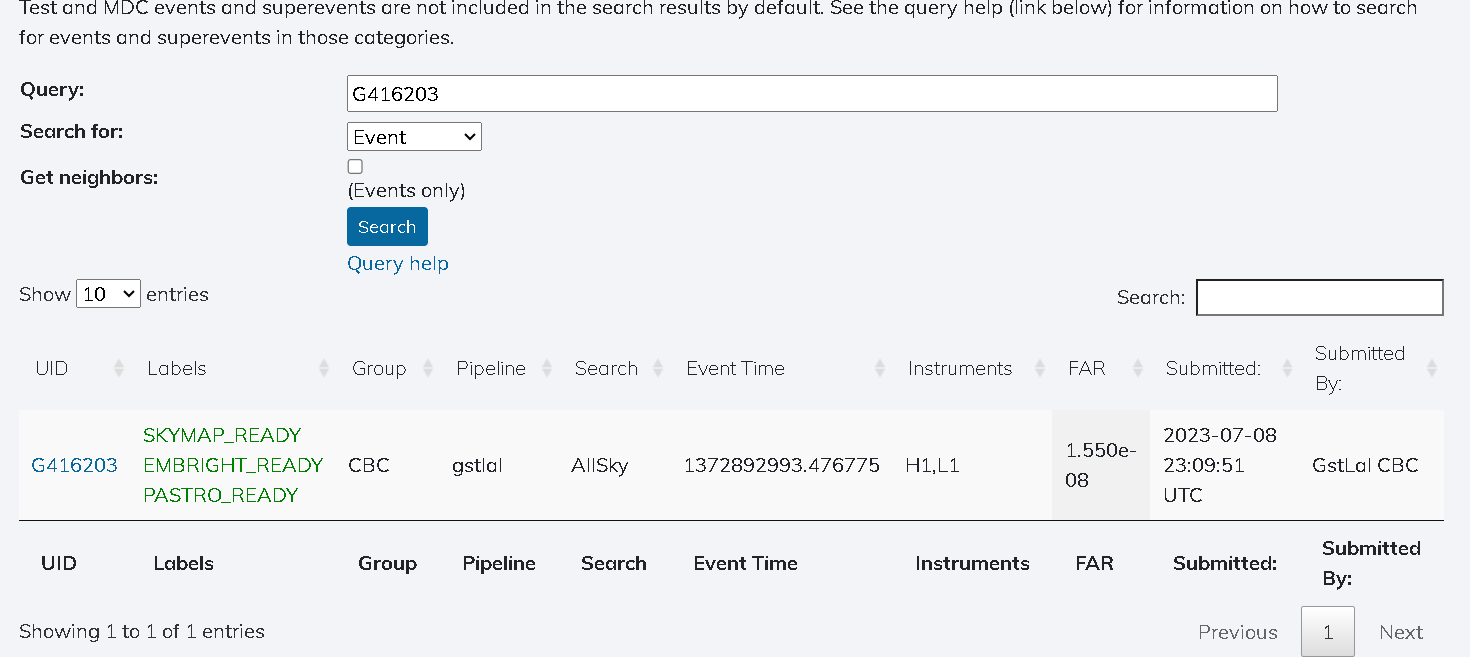
\includegraphics[width=0.6\textwidth]{figs/search.png}
\caption{Search G416203 at GraceDB}
\end{figure}

\subsubsection{See an Event}

Activate the environment. The environment name is that you have set.

\begin{verbatim}
    $ conda activate testlensing
\end{verbatim}

If you know the superevent ID(SID) or the event ID(GID), you can see the property of the (super)event.

\begin{verbatim}
    $ mkdir seeevent
    $ cd seeevent
    $ gracedb get event G416203
\end{verbatim}

\subsubsection{Set Up a TESLA Analysis}

This part is based on Doctor Alvin Li's TESLA guide, the part '\href{https://git.ligo.org/alvin.li/tesla#settting-up-a-tesla-analysis}{Setting up a TESLA analysis}'.

First, initialize the environment and login.

\begin{verbatim}
    $ conda actiavte testlensing
    $ htgettoken -a vault.ligo.org -i igwn
\end{verbatim}

Go to the home directory and make a directory to analyze.

\begin{verbatim}
    $ cd
    $ mkdir Projects
    $ cd Projects
    $ mkdir tesla_o4_runs
    $ cd tesla_o4_runs
    $ mkdir production
    $ cd production
\end{verbatim}

And set the environment.

\begin{verbatim}
    $ cp /home/lensing.o4/Projects/tesla_o4_runs/production/base_config.yml .
    $ ln -s /home/lensing.o4/Projects/tesla_o4_runs/production/S230518h
    $ ln -s /home/lensing.o4/Projects/tesla_o4_runs/production/S230529ay
    $ ln -s /home/lensing.o4/Projects/tesla_o4_runs/production/S230601bf
    $ ln -s /home/lensing.o4/Projects/tesla_o4_runs/production/S230605o
\end{verbatim}

Vim into the base-config file.

\begin{verbatim}
    $ vi base_config.yml
\end{verbatim}

And change those parts:

[basic\_information] -> project\_dir: (The project folder you analyze)

[basic\_information] -> x509\_proxy: ""

[general\_settings] -> group\_user: (your name, ex. albert.einstein)

[general\_settings] -> webdir: /home/(your name)/public\_html/(The folder which has same name as your project directory)

Please see inside the public\_html folder.

Start analysis.

\begin{verbatim}
    $ tesla_initiate_event_analysis --base-config base_config.yml --event G416203
\end{verbatim}

A master config file 'S230708cf\_TESLA-X\_version0\_main\_config.yml' will be generated under the directory 'S230708cf'.

Go to the directory and continue the analysis.

\begin{verbatim}
    $ cd S230708cf/
    $ tesla_initiate_event_analysis \
       --base-config S230708cf_TESLA-X_version0_main_config.yml
\end{verbatim}

If it seems to stop while executing the analysis, it will continue by pressing the Enter key. This case will happen many times.

You can watch the progress as follows in other sessions.

\begin{verbatim}
    $ cd (The project folder you analyze)/S230708cf/TESLA-X_version_0/injection_run/
    $ tail -f (FIX ME)
\end{verbatim}


\end{document}
